\section{Results}

%Two step appraoch of result presentation using two different approaches with different BMs
This section provides an overview of the results while in the next section we discuss them. 

Subfigure \ref{fig:notc_noNS_perf} provides an overview of all portfolios without News Sentiment enhancement and no transaction costs. Subfigure \ref{fig:tc_noNS_perf} provides the same overview but this time the solid line represents the performance without transaction costs while the dotted lines include transaction costs of 25 basis points. Furthermore, both subfigures \ref{fig:notc_noNS_perf} and \ref{fig:tc_noNS_perf} include our benchmarks: "BM Eq" which represents the equally weighted portfolio while "BM Ivp" represents the inverse volatility portfolio. Table \ref{stats} provides summary statistics of the four portfolios as well as for the two benchmarks.

Subfigure \ref{fig:notc_NS_perf} plot the portfolio performance when News Sentiment enhancement is added but with no transaction costs. In subfigure \ref{fig:tc_NS_perf} the dotted lines include transaction costs of 25 basis points. 


% STATISTICS TABLE
\begin{table}[h]
\centering
    \begin{tabular}{lcccccc}
                         & Single & Complete & Average & Ward  & BM Ivp & BM Eq  \\
    \midrule
    Geometric Average Excess Return      & 0.39   & 0.45     & 0.39    & 0.5   & 0.25   & 0.4   \\
Geometric Average Total Return   & 0.45   & 0.49     & 0.43    & 0.54  & 0.3    & 0.45  \\
Arithmetic Average Total Return & 0.46   & 0.49     & 0.44    & 0.54  & 0.29   & 0.46  \\
Arithmetic Average Excess Return    & 0.42   & 0.47     & 0.41    & 0.52  & 0.25   & 0.44  \\
Standard Deviation Excess Returns         & 2.27   & 2.01     & 2.0     & 2.0   & 0.85   & 2.45  \\
Sharpe Ratio Arithmetic     & 0.63   & 0.8      & 0.7     & 0.9   & 1.04   & 0.61  \\
Sharpe Ratio Geometric      & 0.6    & 0.77     & 0.67    & 0.86  & 1.02   & 0.57  \\
Minimum Excess Return          & -8.13  & -8.74    & -7.59   & -8.03 & -3.2   & -13.0 \\
Maximum Excess Return          & 7.87   & 7.73     & 7.92    & 7.15  & 3.13   & 8.23  \\
Skewness Excess Return         & -0.24  & -0.56    & -0.4    & -0.46 & -0.35  & -1.23 \\
Kurtosis Excess Return         & 2.17   & 2.84     & 2.31    & 2.16  & 1.35   & 5.0  \\
    \bottomrule
    \end{tabular}
    \\[5pt]
     \captionsetup{width=0.925\linewidth}
     \caption[Summary statistics of the four different portfolios together with the two benchmark for no News Sentiment enhancement.]{Summary statistics of the four different portfolios (Single, Complete, Average and Ward) together with the two benchmarks for no News Sentiment enhancement. Data is monthly with the Sharpe Ratios annualized.}
    \label{stats}
\end{table}


% PERFORMANCE NO NS ENHANCEMENT
\newpage
\begin{figure}[H] % "[t!]" placement specifier just for this example
\centering

\begin{subfigure}{0.8\textwidth}%{0.48\textwidth}
\centering
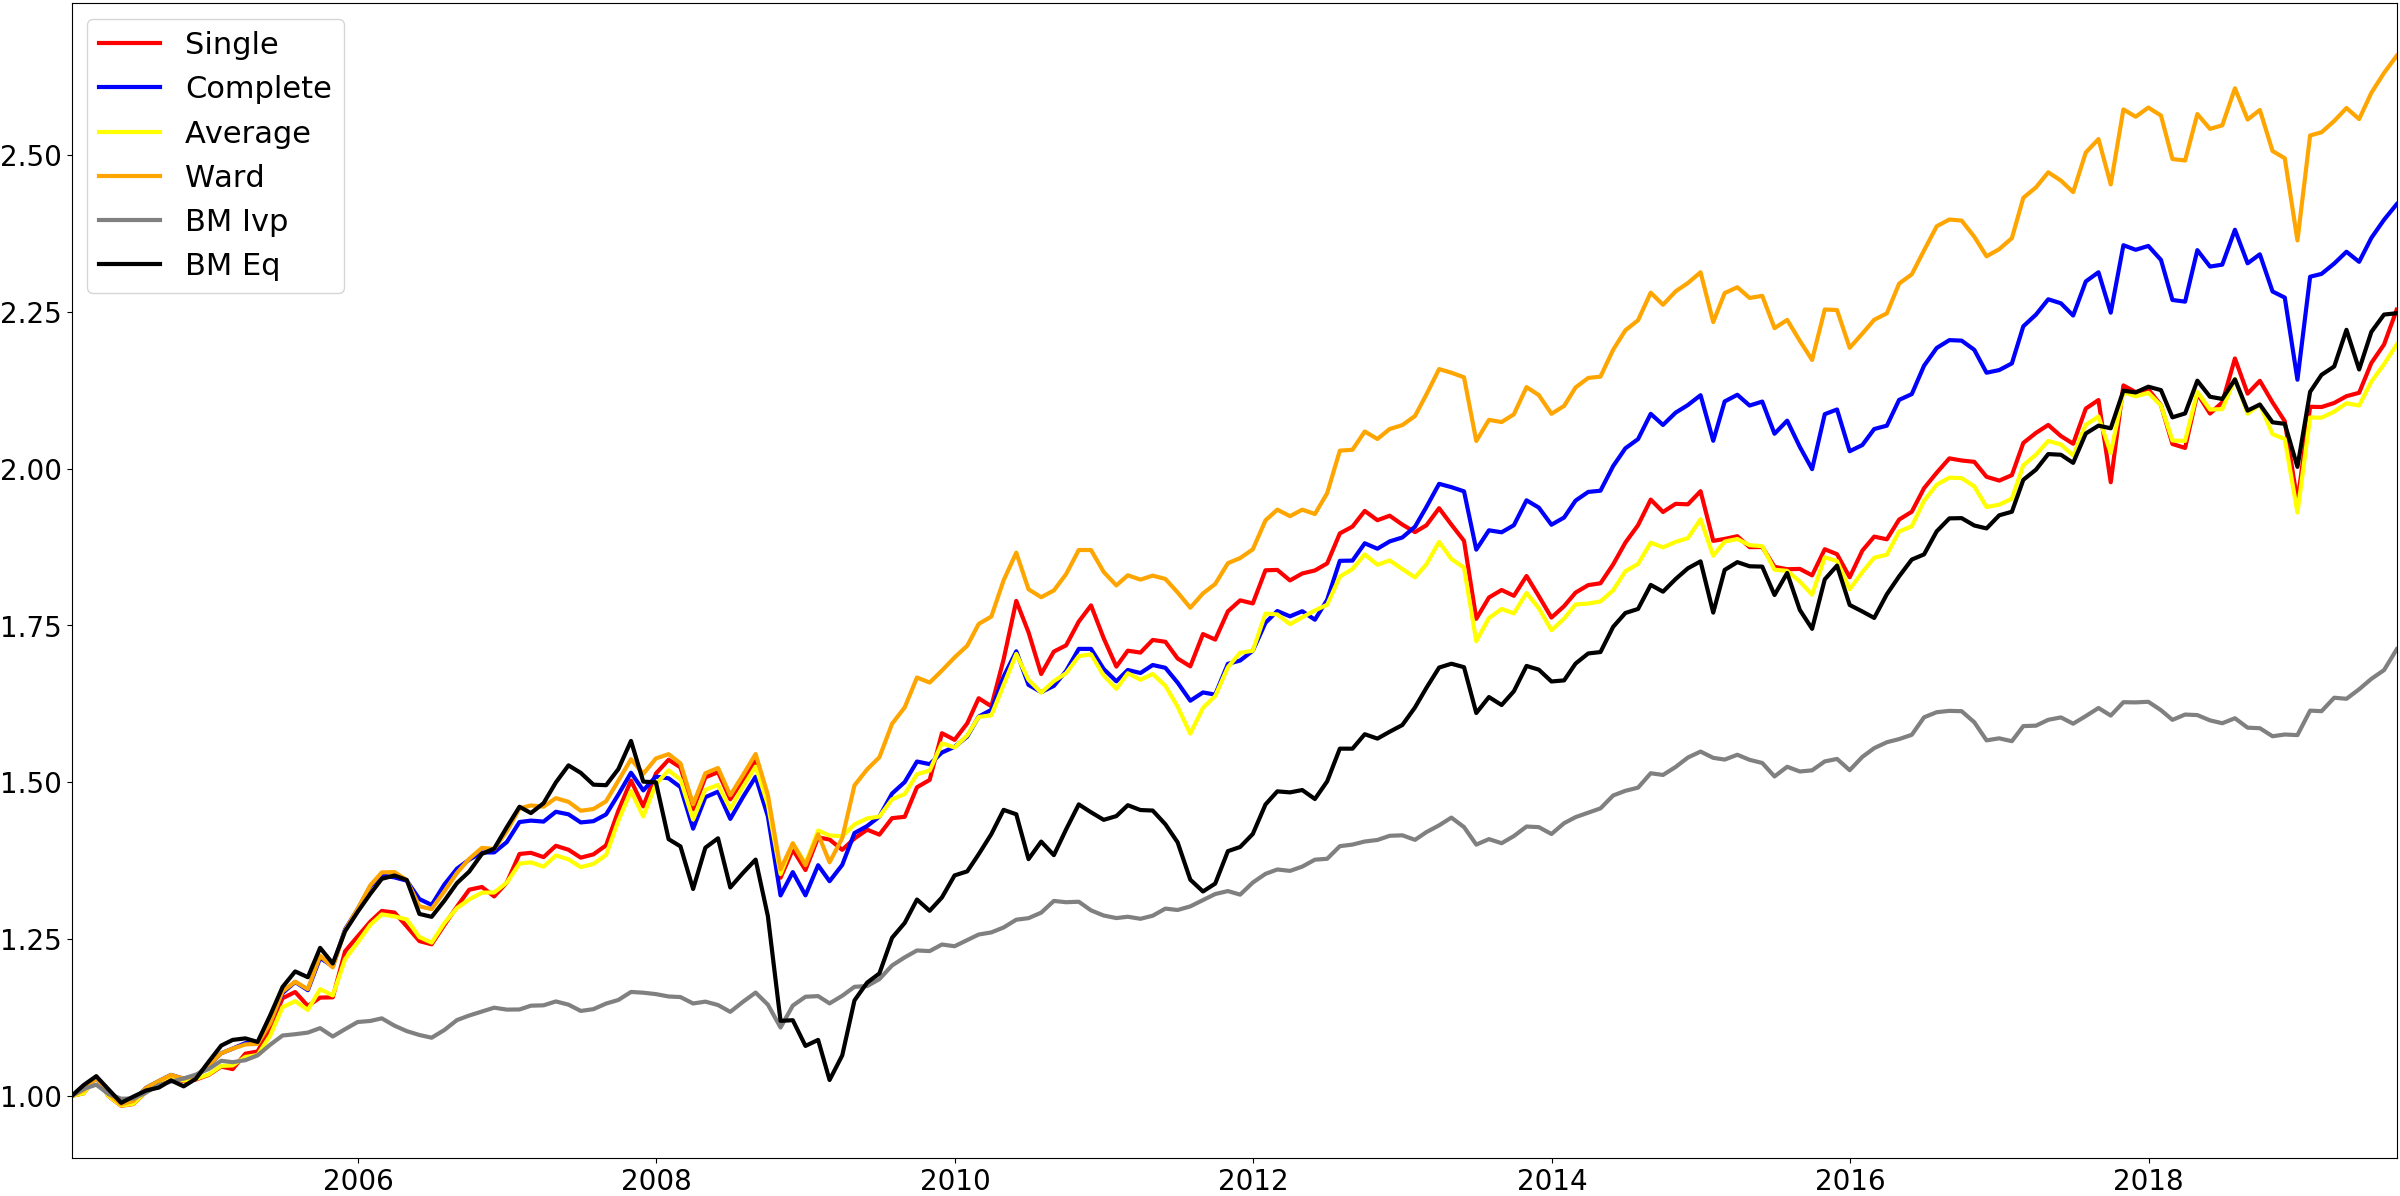
\includegraphics[width=\linewidth]{Plots_and_Tables/perf_noTC_without_NS_F_1_B_0_LB_12_0.png}
\caption{Performance of strategies excluding transaction costs.} \label{fig:notc_noNS_perf}
\end{subfigure}%\hspace*{\fill}

\medskip
\begin{subfigure}{0.8\textwidth}%{0.48\textwidth}
\centering
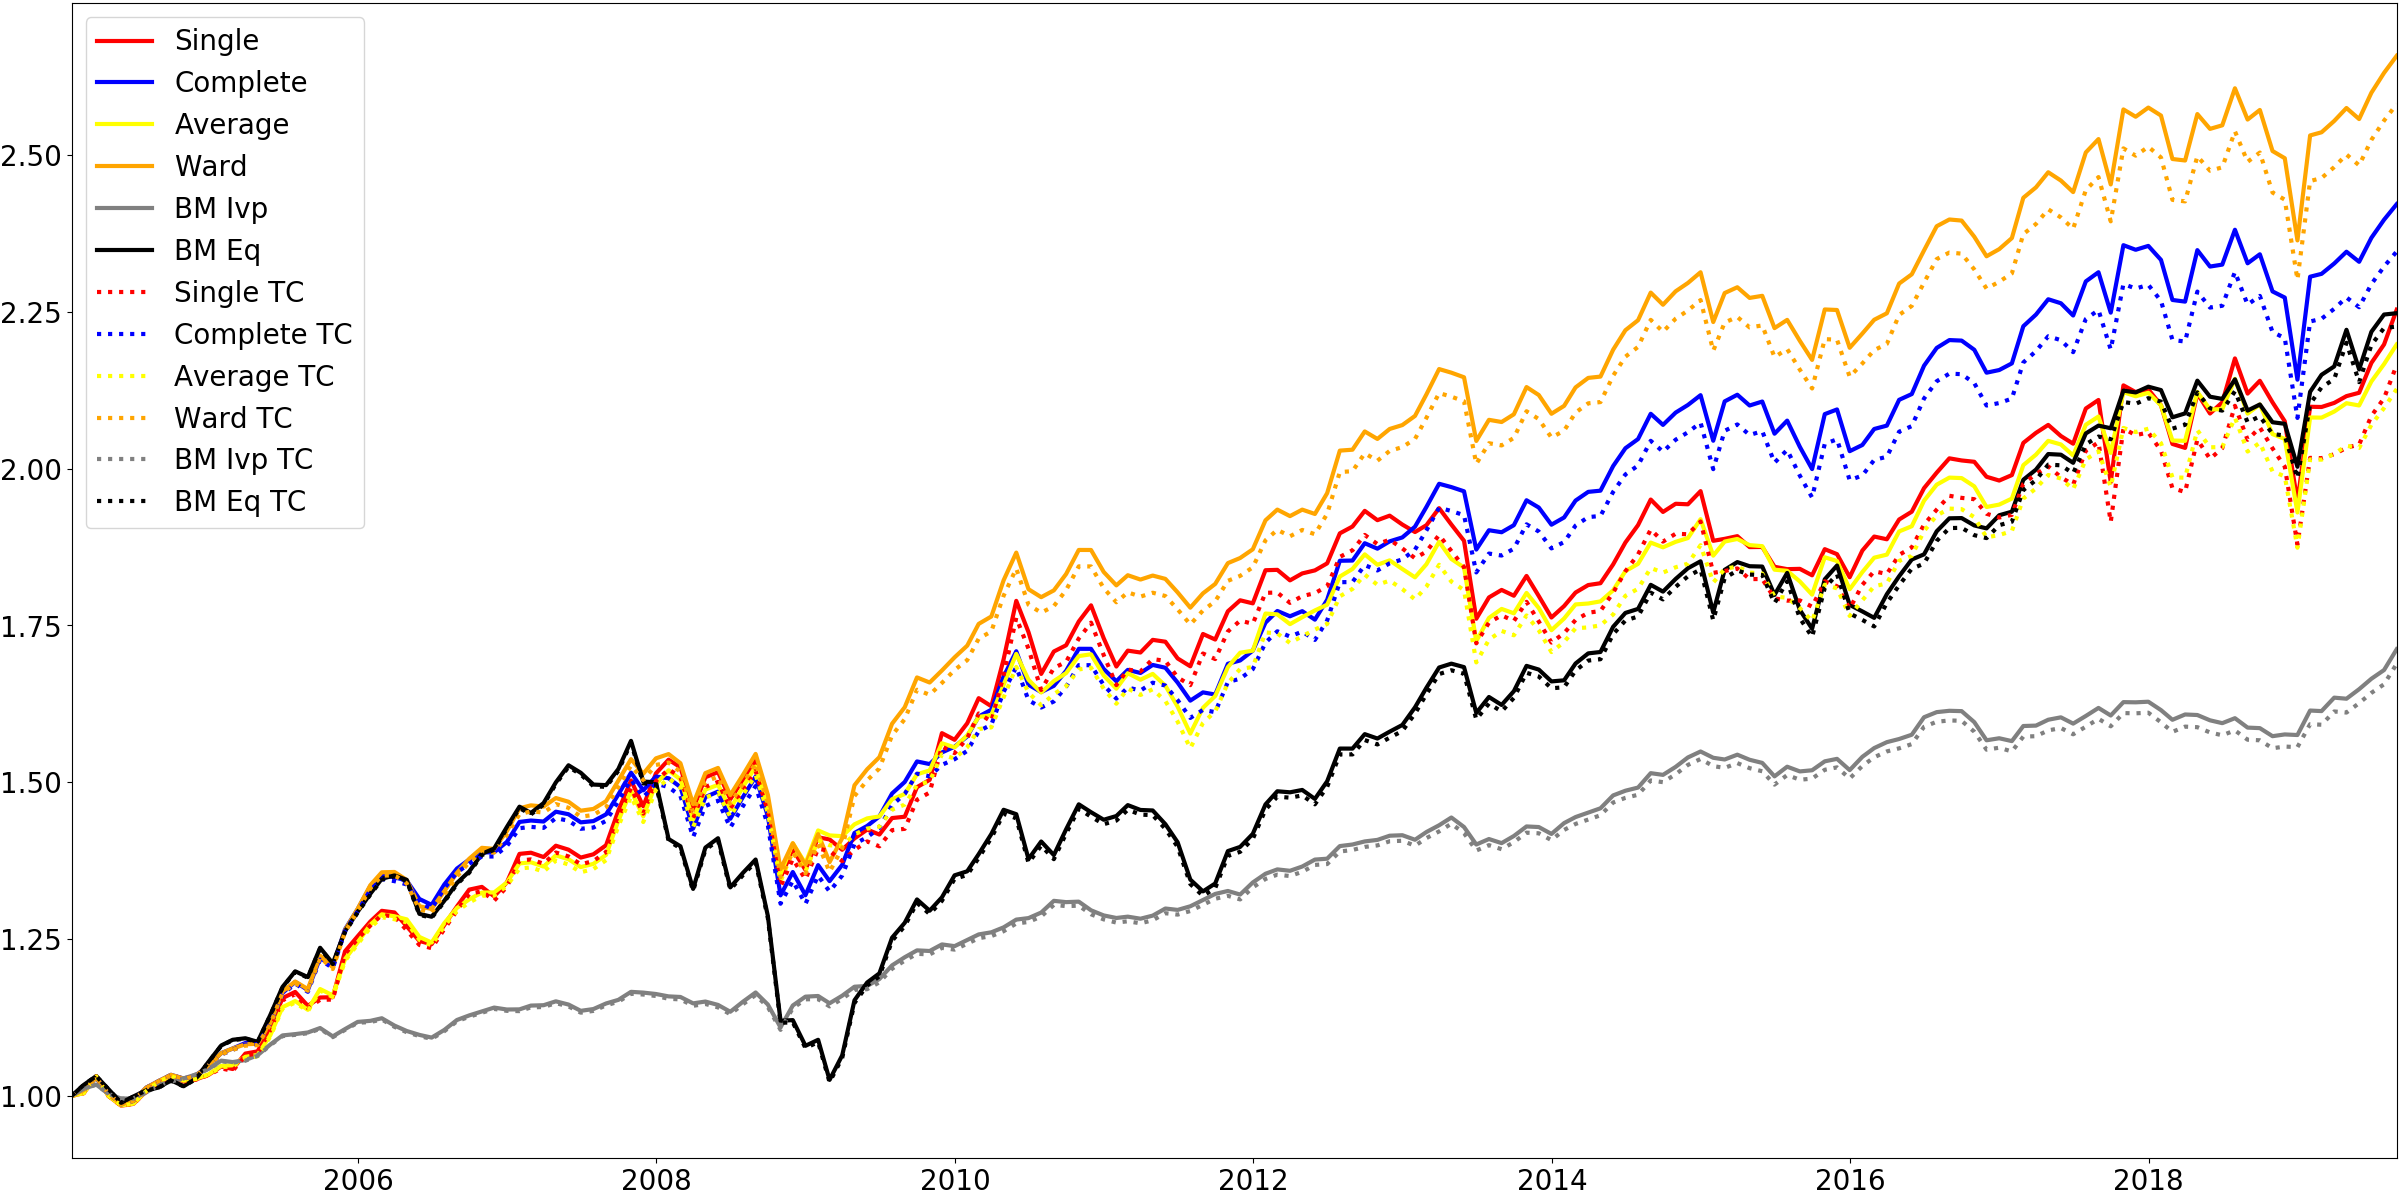
\includegraphics[width=\linewidth]{Plots_and_Tables/perf_noTC_andTC_without_NS_F_1_B_0_LB_12_0.png}
\caption{Performance of strategies including transaction costs.} \label{fig:tc_noNS_perf}
\end{subfigure}%\hspace*{\fill}


% \medskip
% \begin{subfigure}{0.8\textwidth}%{0.48\textwidth}
% \centering
% \includegraphics[width=\linewidth]{Plots_and_Tables/AA_without_NS_F_1_B_0_LB_12_0.png}
% \caption{Comparison of strategy performances with and without transaction costs.} \label{fig:comp_noNS_perf}
% \end{subfigure}%\hspace*{\fill}


\caption{Performance of different strategies without News Sentiment enhancement.} \label{fig:noNS_perf}
\end{figure}
\newpage
\newpage
\begin{figure}[H] % "[t!]" placement specifier just for this example
\centering

\begin{subfigure}{0.8\textwidth}%{0.48\textwidth}
\centering
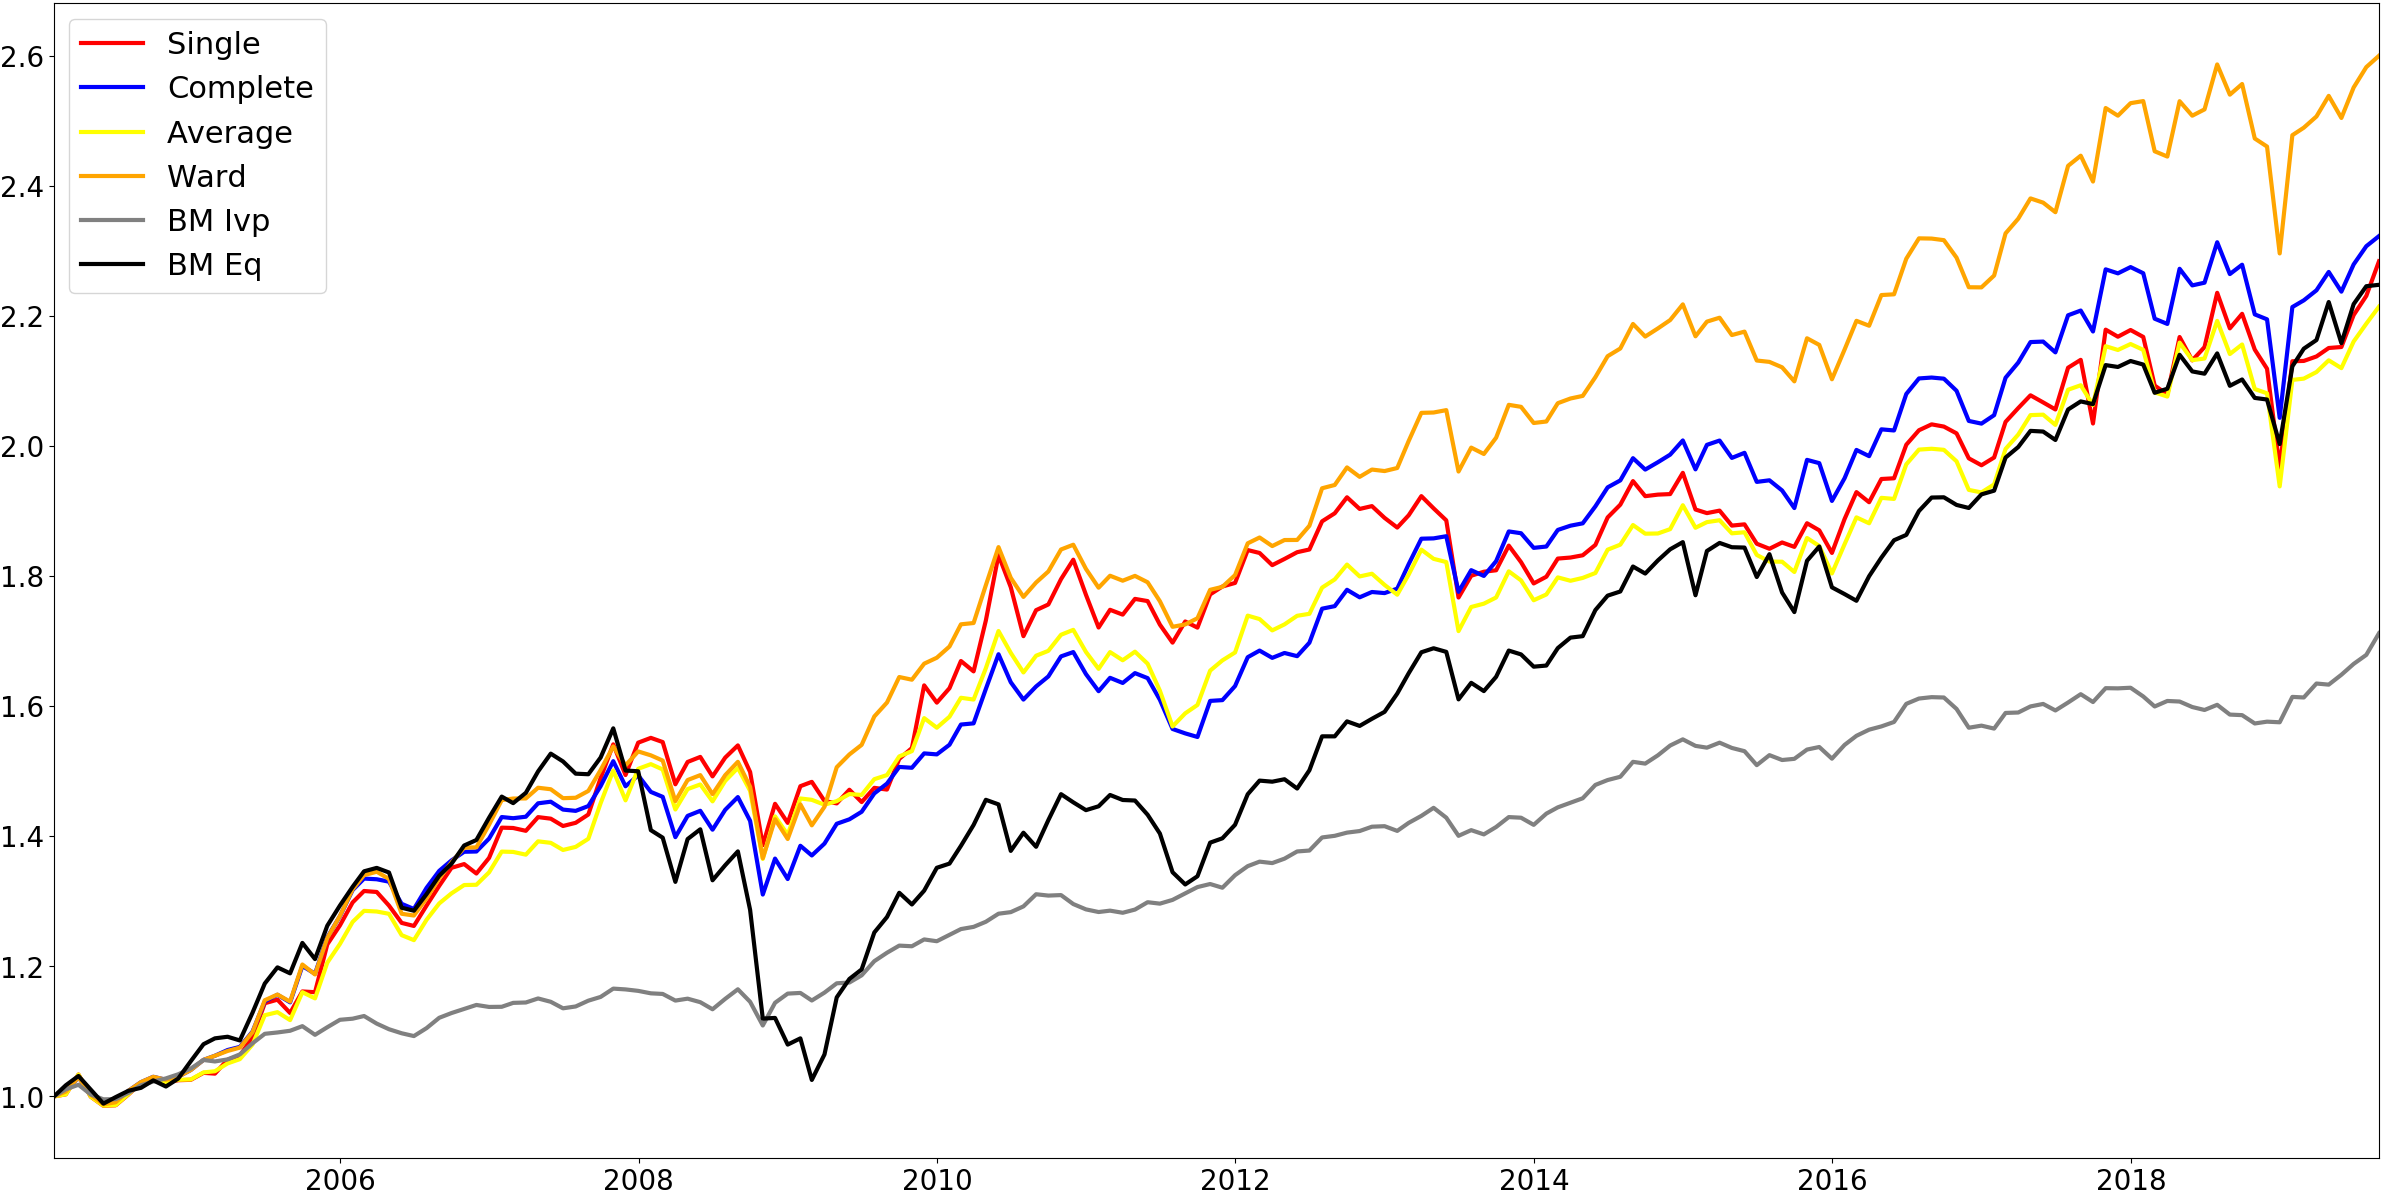
\includegraphics[width=\linewidth]{Plots_and_Tables/perf_noTC_with_NS_F_2_B_0_LB_12_0.png}
\caption{Performance of strategies excluding transaction costs.} \label{fig:notc_NS_perf}
\end{subfigure}%\hspace*{\fill}

\medskip
\begin{subfigure}{0.8\textwidth}%{0.48\textwidth}
\centering
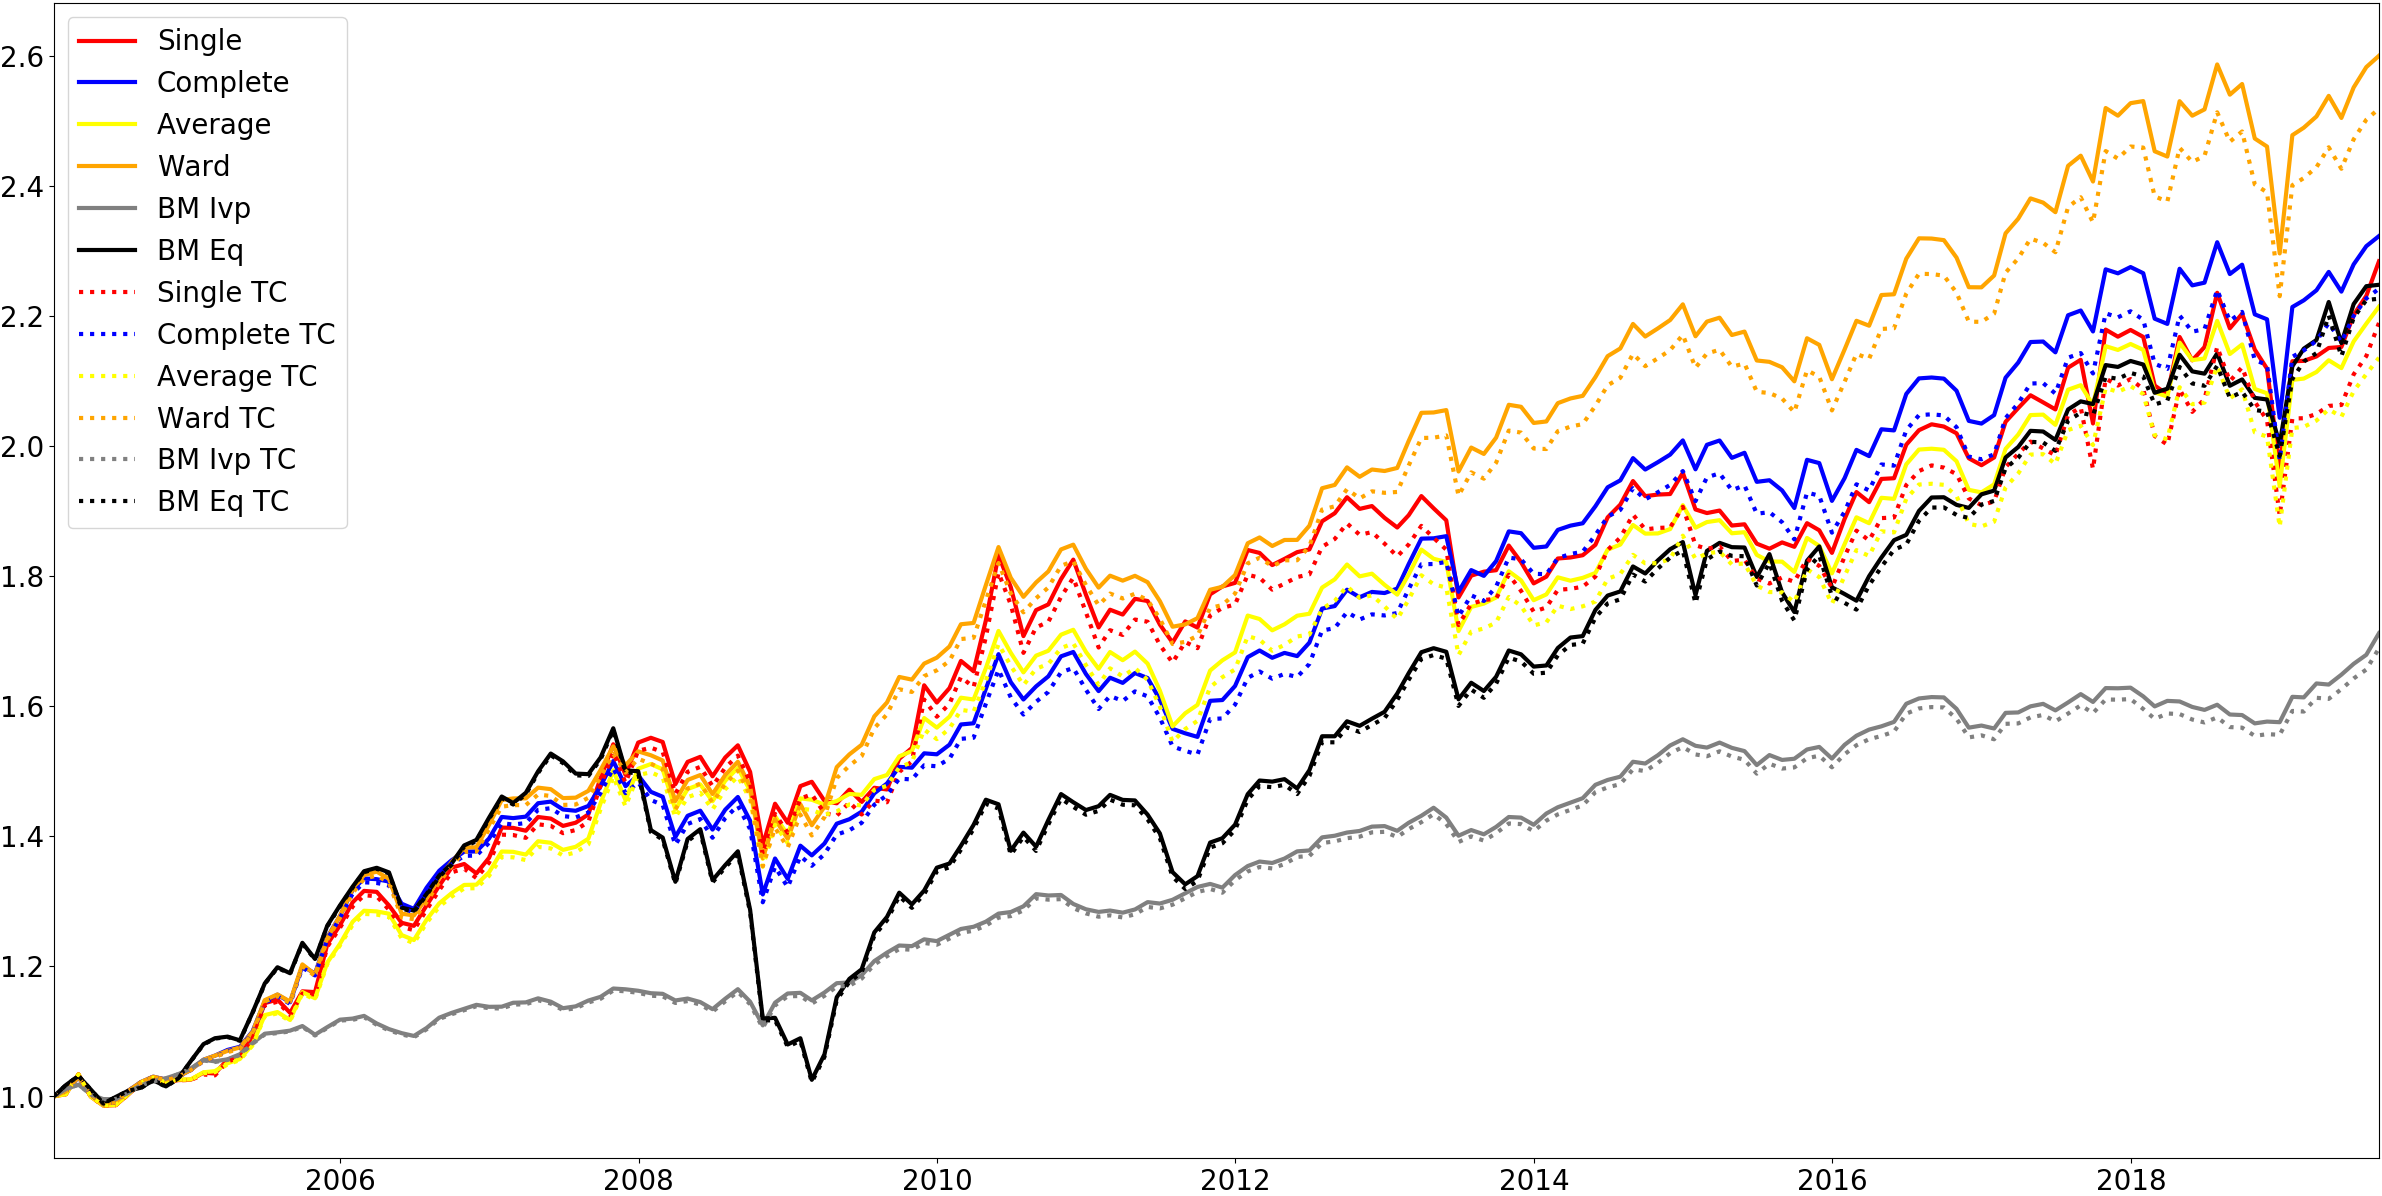
\includegraphics[width=\linewidth]{Plots_and_Tables/perf_noTC_andTC_with_NS_F_2_B_0_LB_12_0.png}
\caption{Performance of strategies including transaction costs.} \label{fig:tc_NS_perf}
\end{subfigure}%\hspace*{\fill}


% \medskip
% \begin{subfigure}{0.8\textwidth}%{0.48\textwidth}
% \centering
% \includegraphics[width=\linewidth]{Plots_and_Tables/AA_with_NS_F_2_B_0_LB_12_0.png}
% \caption{Comparison of strategy performances with and without transaction costs.} \label{fig:comp_NS_perf}
% \end{subfigure}%\hspace*{\fill}


\caption{Performance of different strategies with News Sentiment enhancement.} \label{fig:noNS_perf}
\end{figure}
\newpage
%\newpage
\begin{center}

\begin{figure}[H] % "[t!]" placement specifier just for this example
\centering
\begin{subfigure}{1\textwidth}%{0.48\textwidth}
\centering

\includegraphics[width=\linewidth]{Plots_and_Tables/AA_step1_F_1_B_0_LB_12.png}
\caption{Allocation without News Sentiment enhancement.} \label{fig:notc_NS_perf}
\end{subfigure}%\hspace*{\fill}

\medskip
\begin{subfigure}{1\textwidth}%{0.48\textwidth}
\centering
\includegraphics[width=\linewidth]{Plots_and_Tables/AA_step1_F_2_B_0_LB_12.png}
\caption{Allocation with News Sentiment enhancement.} \label{fig:tc_NS_perf}
\end{subfigure}%\hspace*{\fill}

\caption{Comparison of allocations of strategies with an without NS enhancement.} \label{fig:noNS_perf}
\end{figure}

\end{center}
\newpage




